\documentclass[conference]{IEEEtran}
\IEEEoverridecommandlockouts%

\usepackage[utf8]{inputenc}
\usepackage[T1]{fontenc}
\usepackage[brazilian,english]{babel}
\usepackage{amsmath}
\usepackage{array}
\usepackage{booktabs}
\usepackage{graphicx}
\usepackage{bookmark}
\usepackage{eso-pic}
\usepackage[section]{placeins}
\usepackage{tikz}
\usepackage{listings}
\usepackage{hyperref}
\usepackage{url}

\hypersetup{colorlinks=true,linkcolor=blue,urlcolor=blue,citecolor=blue}

\lstset{basicstyle=\ttfamily\scriptsize, breaklines=true, columns=fullflexible,
        frame=single, framerule=0.3pt, xleftmargin=0pt, aboveskip=4pt, belowskip=2pt}

% ---------------------------------------------------------------
% Author data
% ---------------------------------------------------------------
\newcommand{\authorName}{Navinchandry Bittencourt Ruas}
\newcommand{\authorId}{241034353}
\newcommand{\authorEmail}{241034353@aluno.unb.br}

% Watermark on the background of every page.
\AddToShipoutPictureBG{%
\begin{tikzpicture}[remember picture,overlay]
\node[opacity=0.06,inner sep=0pt] at (current page.center) {
\includegraphics[width=0.48\paperwidth]{figures/unb-logo-square.png}};
\end{tikzpicture}%
}

\title{%

\includegraphics[width=0.95\textwidth]{figures/unb-logo-wide.jpg}\\[-0.8ex]
\vspace{0.4ex}
A Two-Pass Assembler and Linker for a Hypothetical Machine: Design, Implementation and Validation in C++}

\author{%
\IEEEauthorblockN{\authorName}
\IEEEauthorblockA{Department of Computer Science\\
University of Brasília\\
Student ID: \authorId\\
\authorEmail}
}

\begin{document}
\maketitle

\begin{abstract}
This paper describes the design and implementation of a two-pass assembler and a linker for the symbolic language of a 14-instruction hypothetical machine, written in C++17 for the CIC0104 Basic Software course. The assembler performs lexical, syntactic and semantic analysis, supports the \texttt{SPACE}, \texttt{CONST}, \texttt{EQU} and \texttt{IF} directives and \texttt{LABEL + N} addressing, and reports every error in the file, with line and type, before emitting a text object. The linker merges up to three modules, relocating addresses and resolving external symbols. Validation combined 81 automated checks with hand-computed expectations, runs on the course simulator, differential testing against 3,000 random valid programs and fuzzing under memory sanitizers; all succeeded, and the object produced for the reference example is byte-identical to the one provided.
\end{abstract}

\noindent Keywords: assembler, linker, two-pass, lexical analysis, relocation, system software

% ===============================================================
\section{Introduction}
Assemblers and linkers are the foundation of the program translation chain: the former converts symbolic code into machine code and the latter combines separate modules into an executable~\cite{beck,levine}. Implementing them consolidates the concepts of lexical, syntactic and semantic analysis, symbol tables and relocation~\cite{aho}.

The goal of this work, set by the course assignment~\cite{enunciado}, is to build in C/C++ (i)~a \texttt{montador} (assembler) program that translates the hypothetical symbolic language into a text-format object, identifying lexical, syntactic and semantic errors, and (ii)~a \texttt{ligador} (linker) program that, calling the assembler internally, produces a \texttt{.LIG} executable from up to three modules. The implementation, in C++17~\cite{cpp17}, has about 1,320 lines and no external dependencies. The source code is available at \url{https://github.com/naviNBRuas/HypoForge}.

% ===============================================================
\section{Background}
\subsection{The hypothetical machine}
The machine has an accumulator and 14 instructions (Table~\ref{tab:isa}). Each instruction takes one opcode word followed by zero to two addresses. Programs have a \texttt{TEXT} section (instructions) and a \texttt{DATA} section (\texttt{CONST} and \texttt{SPACE}); in the object, data always comes after code.

\begin{table}[!htbp]
\centering
\caption{Instructions of the hypothetical machine}\label{tab:isa}
\begin{tabular}{p{2.5cm} p{1.2cm} p{3.3cm}}
\toprule
\textbf{Instruction} & \textbf{Opcode} & \textbf{Size (words)}\\
\midrule
ADD, SUB, MULT, DIV & 1--4 & 2\\
JMP, JMPN, JMPP, JMPZ & 5--8 & 2\\
COPY & 9 & 3\\
LOAD, STORE & 10, 11 & 2\\
INPUT, OUTPUT & 12, 13 & 2\\
STOP & 14 & 1\\
\bottomrule
\end{tabular}
\end{table}

\subsection{Two-pass assembly}
References to labels defined further ahead prevent code from being generated immediately. The two-pass algorithm solves this: the first pass walks the source, computes the size of each statement and fills the symbol table; the second, with every address known, generates the words~\cite{beck}.

\subsection{Linking and relocation}
Modules are assembled independently, with addresses relative to their own start. The linker adds a \emph{base} to each module (the sum of the sizes of the previous ones) to every word that represents a local address, and fills references to \texttt{EXTERN} symbols with the addresses defined by \texttt{PUBLIC} in other modules~\cite{levine}.

% ===============================================================
\section{Design and Implementation}
\subsection{Overview}
The code is organised in small modules: instruction table, lexer, assembler, object formats and linker, shared by two executables. Fig.~\ref{fig:architecture} shows the assembler flow.

\begin{figure}[!htbp]
\centering
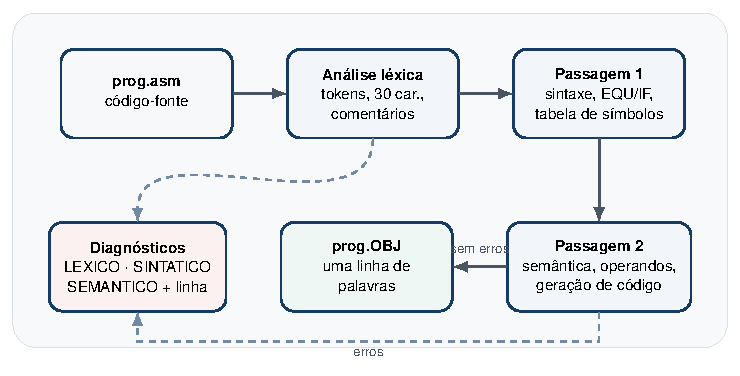
\includegraphics[width=0.98\linewidth]{figures/fig1-architecture.pdf}
\caption{Assembler flow: lexical analysis, two passes and object generation; errors are accumulated and printed at the end.}\label{fig:architecture}
\end{figure}

\subsection{Lexical analysis}
Each line is cut at the \texttt{;} symbol and split into identifiers, numbers and the symbols \texttt{:}, \texttt{+}, \texttt{-} and comma. Identifiers are upper-cased, making the language case-insensitive, and tabs and extra blanks are ignored. Lexical errors are: characters outside the alphabet, identifiers longer than 30 characters and tokens starting with a digit (such as \texttt{1ABC} and \texttt{0x10}, since \texttt{CONST} accepts decimal only).

\subsection{First pass: syntax and symbols}
For each line, \texttt{label:}, the mnemonic and the operands are recognised, checking the number of operands. A label alone on a line stays pending and is attached to the next statement. Labels are recorded with section-relative addresses; \texttt{EQU} is evaluated immediately and a false \texttt{IF} discards the following line. Lines with a lexical error receive no further syntactic analysis, avoiding cascading errors.

\subsection{Second pass: semantics and code}
With the text size known, data labels receive \texttt{address + text size}, which allows the \texttt{DATA} section to come before or after \texttt{TEXT}. \texttt{LABEL + N} operands are resolved and the semantic checks are applied (Table~\ref{tab:errors}). The whole file is always analysed; errors are sorted by line and, if there is any, no \texttt{.OBJ} is written.

\begin{table}[!htbp]
\centering
\caption{Detected errors by class}\label{tab:errors}
\begin{tabular}{p{2.1cm} p{4.9cm}}
\toprule
\textbf{Class} & \textbf{Examples}\\
\midrule
LEXICO & invalid character; identifier $>$ 30; token starting with a digit\\
SINTATICO & wrong operand count; invalid instruction/directive; comma in \texttt{COPY}; two labels\\
SEMANTICO & missing or repeated label; missing \texttt{TEXT}; write to \texttt{CONST}; jump to data; access beyond the area reserved by \texttt{SPACE}/\texttt{CONST}; division by constant 0; \texttt{BEGIN} without \texttt{END}\\
\bottomrule
\end{tabular}
\end{table}

\subsection{Object formats and linker}
The assembler object is one line of blank-separated words, program first and then data, identical to the format of the reference example. When called by the linker (\texttt{--modular} option), the assembler adds tables of definitions (\texttt{D}), external uses (\texttt{U}) and one relocation bit per word (\texttt{R}). The linker (i)~computes the bases, (ii)~builds the global symbol table, (iii)~adds the base to the marked words and (iv)~adds the global address of the symbol to each external use. Duplicate definitions and undefined externals abort linking. Fig.~\ref{fig:linking} illustrates the result for the two-module example.

\begin{figure}[!htbp]
\centering
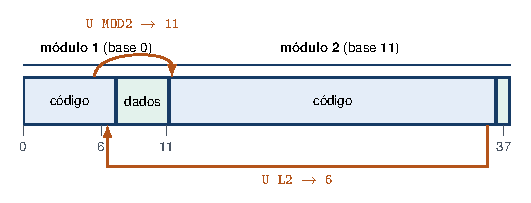
\includegraphics[width=0.98\linewidth]{figures/fig2-linking.pdf}
\caption{Layout of the linked executable (37 words) and the two resolved external references.}\label{fig:linking}
\end{figure}

% ===============================================================
\section{Tests and Results}
\subsection{Methodology}
The suite (\texttt{make test}) comprises 81 checks (Table~\ref{tab:tests}). For valid programs, the object is compared byte by byte against hand-computed expectations, and the provided example is compared against the reference object. For invalid programs, the list of line/error-type pairs is compared. Assembled and linked programs are also run on the course simulator, and the command-line checks cover file names with dots, blanks and upper-case extensions, wrong argument counts and the removal of stale outputs after a failure.

Beyond the course examples, the cases target inputs a grader is likely to try: labels alone on a line followed by comments and blank lines, identifiers of exactly 30 and 31 characters, \texttt{LABEL+N} without blanks, \texttt{COPY A,B}, hexadecimal, fractional and out-of-range constants, accented characters, reserved words as labels, nested \texttt{IF}, a UTF-8 BOM and CRLF or CR-only line endings. Two stress tools complement the suite (\texttt{make stress}): a differential test that generates 3,000 random valid programs, computes their objects independently and requires byte-for-byte equality, and a fuzzer that feeds 6,000 random or mutated programs and 600 random links to the tools. Under AddressSanitizer and UBSan, neither the suite nor the fuzzer revealed crashes or memory errors.

\begin{table}[!htbp]
\centering
\caption{Test-suite summary}\label{tab:tests}
\begin{tabular}{p{2.6cm} p{0.9cm} p{3.2cm}}
\toprule
\textbf{Category} & \textbf{Cases} & \textbf{Result}\\
\midrule
Valid programs & 25 & identical object\\
Invalid programs & 28 & correct lines and types\\
Linking & 13 & \texttt{.LIG}, output and errors\\
Simulator runs & 6 & expected output\\
Command line & 9 & names, exit codes\\
\midrule
\textbf{Total} & \textbf{81} & \textbf{81 passed}\\
\bottomrule
\end{tabular}
\end{table}

\subsection{Assembling a valid program}
The program \texttt{bin.asm} reads an integer and prints its binary digits (least significant first). The generated object matches the reference one:
\begin{lstlisting}
$ ./montador examples/bin.asm
Montagem concluida: examples/bin.OBJ (32 palavras)
$ cat examples/bin.OBJ
12 29 10 29 4 28 11 30 3 28 11 31 10 29 2 31 11 31
13 31 9 30 29 10 29 7 4 14 2 0 0 0
\end{lstlisting}

\subsection{Error detection}
For the assignment example, in which label \texttt{N3} is not declared, every occurrence is reported in a single run (the tool messages are in Portuguese, as the course requires the \texttt{LEXICO}, \texttt{SINTATICO} and \texttt{SEMANTICO} classes):
\begin{lstlisting}
[ERRO SEMANTICO] linha 11: rotulo 'N3' nao declarado
    11 | COPY N2 N3
[ERRO SEMANTICO] linha 12: rotulo 'N3' nao declarado
    12 | COPY N3 N3
[ERRO SEMANTICO] linha 13: rotulo 'N3' nao declarado
    13 | OUTPUT N3
\end{lstlisting}

\subsection{Linking modules}
Module~1 reads the number and jumps to \texttt{MOD2}; module~2 runs the loop and returns to \texttt{L2}. The linked executable produces the same outputs as the single-module program for every tested input (for example, 13 yields 1, 0, 1, 1):
\begin{lstlisting}
$ ./ligador examples/modulo1.asm examples/modulo2.asm
  modulo examples/modulo1.asm: base 0, 11 palavras
  modulo examples/modulo2.asm: base 11, 26 palavras
Ligacao concluida: examples/modulo1.LIG (37 palavras)
\end{lstlisting}
A three-module case (adding a constant to a value read from input) and linking-error cases were also tested.

% ===============================================================
\section{Discussion}
\subsection{Interpretation decisions}
The assignment leaves some points open, resolved as follows. Both \texttt{SECAO} and \texttt{SECTION} are accepted, since the text and the examples disagree. \texttt{COPY} with a comma is a syntactic error, because test files will not be fixed. A hexadecimal \texttt{CONST} is a lexical error (decimal only). The object ends with a blank after each word and no final newline, reproducing the provided example. \texttt{END} does not stop reading, since the module example places \texttt{SECTION DATA} after it. Beyond the six error classes listed in the assignment, classic checks were implemented (write to a constant, division by constant zero, incompatible label type, access beyond the reserved area). A UTF-8 BOM and CR-only line endings are accepted, and a failed run removes any stale \texttt{.OBJ} or \texttt{.LIG} left by an earlier one.

\subsection{Inconsistencies in the examples}
The course's sample modular object reports \texttt{L2} at address 7, but the labelled \texttt{STOP} instruction is at address 6; it names \texttt{TEMP\_DATA} a symbol declared as \texttt{TMP\_DATA}; and it carries 9 relocation bits for 11 words. The modular format adopted here keeps the same \texttt{D/U/R} scheme, but with one bit per word and checked addresses.

\subsection{Limitations}
The linker accepts at most three modules, as the assignment states, and assumes execution starts in the first module. Bounds on \texttt{LABEL + N} are checked only for local data; an offset applied to an \texttt{EXTERN} symbol cannot be checked by the assembler.

% ===============================================================
\section{Conclusions}
A two-pass assembler and a linker that meet the specification were implemented: text-format output with the file name's extension changed to \texttt{.OBJ}, full-file analysis with errors by line and type, \texttt{EQU}/\texttt{IF} support and linking of up to three modules with relocation. Automated validation and the use of the course simulator indicate correct behaviour in the covered scenarios, including byte-for-byte identity with the reference object.

As future work we suggest: (i)~bounds checking of external offsets at link time; (ii)~a listing mode with addresses and code side by side; and (iii)~a configurable entry point in the linker.

% ---------------------------------------------------------------
% REFERENCES
% ---------------------------------------------------------------
\begin{thebibliography}{10}
\bibitem{aho} A. V. Aho, M. S. Lam, R. Sethi and J. D. Ullman, \emph{Compilers: Principles, Techniques, and Tools}, 2nd ed. Pearson Addison-Wesley, 2006.
\bibitem{beck} L. L. Beck, \emph{System Software: An Introduction to Systems Programming}, 3rd ed. Addison-Wesley, 1997.
\bibitem{levine} J. R. Levine, \emph{Linkers and Loaders}. Morgan Kaufmann, 1999.
\bibitem{enunciado} University of Brasília, Department of Computer Science, ``Practical Assignment 1 --- CIC0104 Software Básico (Basic Software), class T02,'' course assignment.
\bibitem{cpp17} ISO/IEC 14882:2017, \emph{Programming Languages --- C++}, 2017.
\end{thebibliography}

\end{document}
